With the new flurry of interest in the scaling behavior of CASTRO, we've run some tests on Franklin.
\section{Sod Problem in 3D}
We ran the Sod problem (inputs-test2-x) for 10 time steps with max\_level = 0 on 4, 32, 256, 2048 and 16384 processors. This is a gamma-law gas with no reactions and one species. On 4 processors the base grid was 512x128x128; for each factor of 8 increase in processors we doubled the number of cells in each direction. We set max\_grid\_size = 64 for all cases, resulting in 256 grids per processor. (Thus for perfect scaling we would expect this plot to be flat.) 
%%%%%%%%%%%%%%%%%%%%%%%%%%%%%%%%%
\begin{figure}[h]
\centering
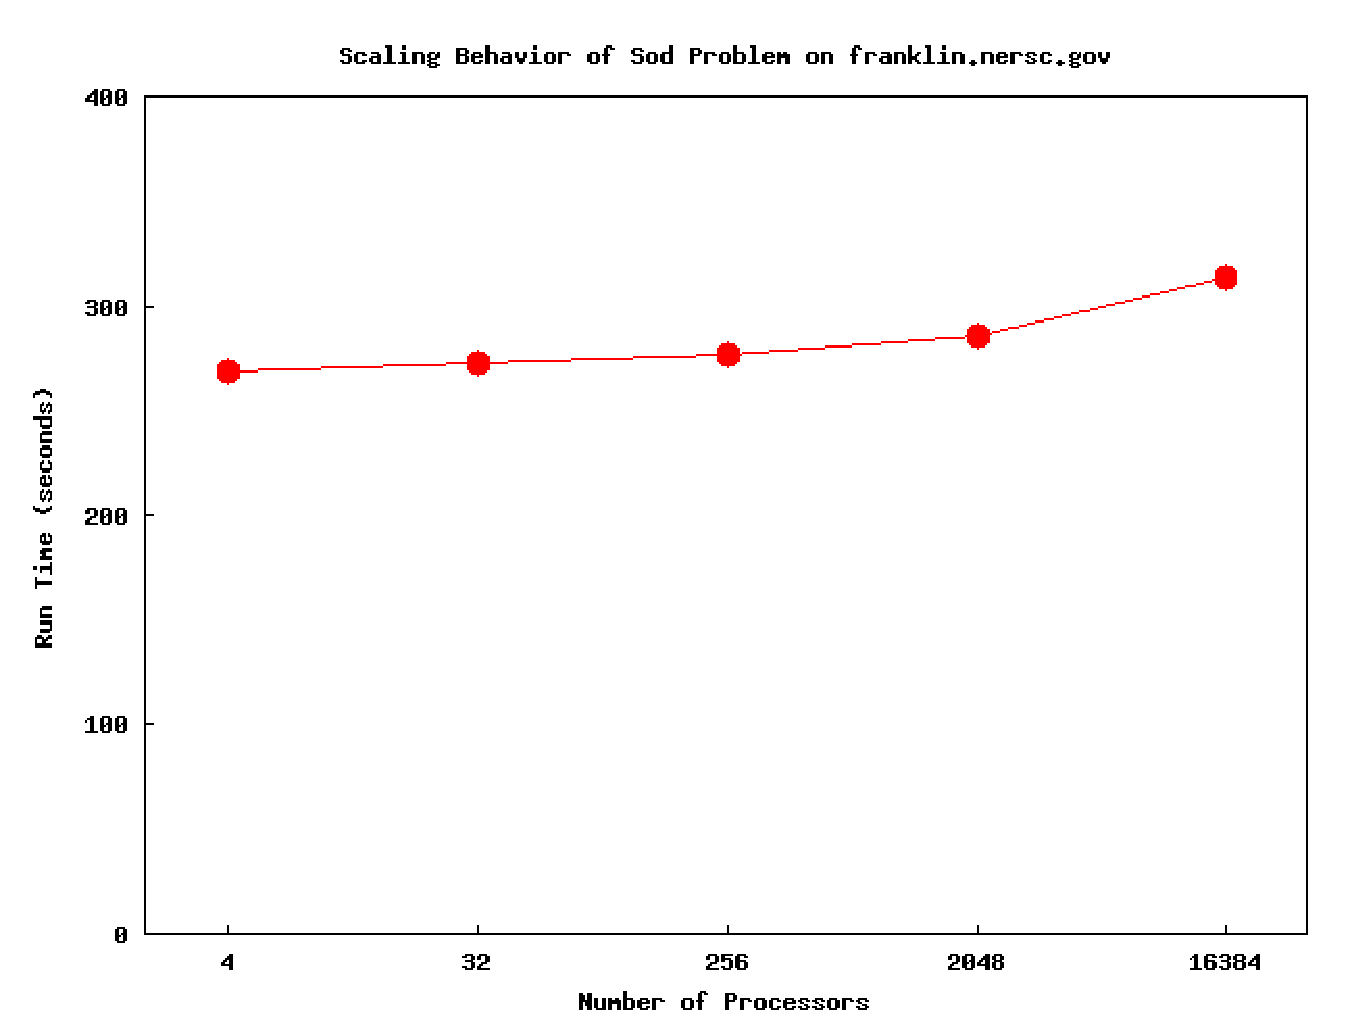
\includegraphics[width=5in]{Scaling/Sod_scaling}
\caption{Scaling behavior of Sod problem on franklin.nersc.gov}
\end{figure}
%%%%%%%%%%%%%%%%%%%%%%%%%%%%%%%%%
\section{White Dwarf in 3D}\label{Sec:White Dwarf in 3D}
This test was performed on 6/1/09 using ScalingTest/inputs.nog, inputs.g3, inputs.g5, inputs.g3.2levels, and inputs.g5.2levels on jaguarpf.  Here we interpolated a 1D initial model of a white dwarf onto a 3D Cartesian grid and ran 5 time steps. This problem used the Helmholtz EOS with no reactions, no thermal diffusion, and three species.  

We ran this problem on 8, 64, 512, 4096, 13824, 32768, and 64000 processors.  The base grid size, respectively, was $128^3, 256^3, 512^3, 1024^3, 1536^3, 2048^3$, and $2560^3$.  We ran with no gravity (castro.do\_grav = 0), gravity type 3 (Poisson solver using multigrid) and gravity type 5 (1D integration of the averaged radial density to define a monopole approximation for gravity), each with max\_level=0.  We also ran with gravity types 3 and 5 with max\_level=1.  The fine grid structure had the exact same grid structure as the coarse level and was centered in the domain.  For all cases max\_grid\_size = 64, so there was 1 processor per grid per level.  Thus for perfect scaling we would expect this plot to be flat. 
%%%%%%%%%%%%%%%%%%%%%%%%%%%%%%%%%
\begin{figure}[h]
\centering
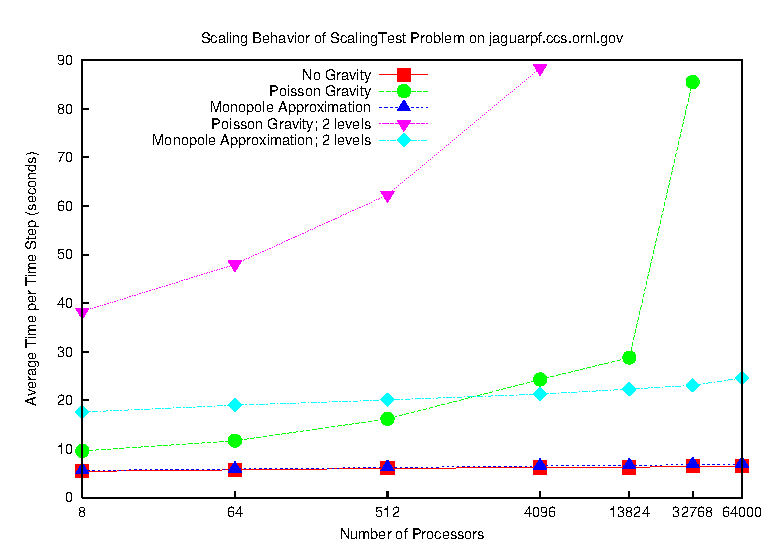
\includegraphics[width=5in]{Scaling/scaling_jaguarpf}
\caption{Scaling behavior of ScalingTest problem on jaguarpf.ccs.ornl.gov}
\end{figure}
%%%%%%%%%%%%%%%%%%%%%%%%%%%%%%%%%
